\documentclass[a4paper,12pt]{report}

%%%%%%%%%%%%%%%%%%%%%%%%%%%%%%%%%
% PACKAGE IMPORTS
%%%%%%%%%%%%%%%%%%%%%%%%%%%%%%%%%
\usepackage[tmargin=2cm,rmargin=1in,lmargin=1in,margin=0.85in,bmargin=2cm,footskip=.2in]{geometry}
\usepackage[none]{hyphenat}
\usepackage{amsmath,amsfonts,amsthm,amssymb,mathtools}
\allowdisplaybreaks
\usepackage{undertilde}
\usepackage{xfrac}
\usepackage[makeroom]{cancel}
\usepackage{mathtools}
\usepackage{bookmark}
\usepackage{enumitem}
\usepackage{kbordermatrix}
\renewcommand{\kbldelim}{(} % Change left delimiter to (
\renewcommand{\kbrdelim}{)} % Change right delimiter to )
\usepackage{hyperref,theoremref}
\hypersetup{
	pdftitle={Assignment},
	colorlinks=true, linkcolor=doc!90,
	bookmarksnumbered=true,
	bookmarksopen=true
}
\usepackage[most,many,breakable]{tcolorbox}
\usepackage{xcolor}
\usepackage{varwidth}
\usepackage{varwidth}
\usepackage{etoolbox}
%\usepackage{authblk}
\usepackage{nameref}
\usepackage{multicol,array}
\usepackage{tikz-cd}
\usepackage[ruled,vlined,linesnumbered]{algorithm2e}
\usepackage{comment} % enables the use of multi-line comments (\ifx \fi) 
\usepackage{import}
\usepackage{xifthen}
\usepackage{pdfpages}
\usepackage{svg}
\usepackage{transparent}
\usepackage{pgfplots}
\pgfplotsset{compat=1.18}
\usetikzlibrary{calc}
\usetikzlibrary{graphs}
\usetikzlibrary{graphs.standard}
% \usetikzlibrary{graphdrawing}

\newcommand\mycommfont[1]{\footnotesize\ttfamily\textcolor{blue}{#1}}
\SetCommentSty{mycommfont}
\newcommand{\incfig}[1]{%
    \def\svgwidth{\columnwidth}
    \import{./figures/}{#1.pdf_tex}
}


\usepackage{tikzsymbols}
% \renewcommand\qedsymbol{$\Laughey$}

\definecolor{commentgreen}{RGB}{2,112,10}
%%
%% Julia definition (c) 2014 Jubobs
%%
\lstdefinelanguage{Julia}%
  {morekeywords={abstract,break,case,catch,const,continue,do,else,elseif,%
      end,export,false,for,function,immutable,import,importall,if,in,%
      macro,module,otherwise,quote,return,switch,true,try,type,typealias,%
      using,while},%
   sensitive=true,%
   alsoother={$},%
   morecomment=[l]\#,%
   morecomment=[n]{\#=}{=\#},%
   morestring=[s]{"}{"},%
   morestring=[m]{'}{'},%
}[keywords,comments,strings]%

\lstset{%
    language        	= Julia,
    basicstyle      	= \ttfamily,
    keywordstyle    	= \bfseries\color{blue},
    stringstyle     	= \color{magenta},
    commentstyle    	= \color{commentgreen},
    showstringspaces	= false,
		numbers						= left,
		tabsize						= 4,
}

\definecolor{stringyellow}{RGB}{227, 78, 48}
%% 
%% Shamelessly stolen from Vivi on Stackoverflow
%% https://tex.stackexchange.com/questions/75116/what-can-i-use-to-typeset-matlab-code-in-my-document
%%
\lstset{language=Matlab,%
    %basicstyle=\color{red},
    breaklines=true,%
    morekeywords={matlab2tikz},
		morekeywords={subtitle}
    keywordstyle=\color{blue},%
    morekeywords=[2]{1}, keywordstyle=[2]{\color{black}},
    identifierstyle=\color{black},%
    stringstyle=\color{stringyellow},
    commentstyle=\color{commentgreen},%
    showstringspaces=false,%without this there will be a symbol in the places where there is a space
    numbers=left,%
		firstnumber=1,
    % numberstyle={\tiny \color{black}},% size of the numbers
    % numbersep=9pt, % this defines how far the numbers are from the text
    emph=[1]{for,end,break},emphstyle=[1]\color{red}, %some words to emphasise
    %emph=[2]{word1,word2}, emphstyle=[2]{style},    
}

%% 
%% Shamelessly stolen from egreg on Stackoverflow
%% https://tex.stackexchange.com/questions/280681/how-to-have-multiple-lines-of-intertext-within-align-environment
%%
\newlength{\normalparindent}
\AtBeginDocument{\setlength{\normalparindent}{\parindent}}
\newcommand{\longintertext}[1]{%
  \intertext{%
    \parbox{\linewidth}{%
      \setlength{\parindent}{\normalparindent}
      \noindent#1%
    }%
  }%
}

%\usepackage{import}
%\usepackage{xifthen}
%\usepackage{pdfpages}
%\usepackage{transparent}

%%%%%%%%%%%%%%%%%%%%%%%%%%%%%%
% SELF MADE COLORS
%%%%%%%%%%%%%%%%%%%%%%%%%%%%%%
\definecolor{myg}{RGB}{56, 140, 70}
\definecolor{myb}{RGB}{45, 111, 177}
\definecolor{myr}{RGB}{199, 68, 64}
\definecolor{mytheorembg}{HTML}{F2F2F9}
\definecolor{mytheoremfr}{HTML}{00007B}
\definecolor{mylenmabg}{HTML}{FFFAF8}
\definecolor{mylenmafr}{HTML}{983b0f}
\definecolor{mypropbg}{HTML}{f2fbfc}
\definecolor{mypropfr}{HTML}{191971}
\definecolor{myexamplebg}{HTML}{F2FBF8}
\definecolor{myexamplefr}{HTML}{88D6D1}
\definecolor{myexampleti}{HTML}{2A7F7F}
\definecolor{mydefinitbg}{HTML}{E5E5FF}
\definecolor{mydefinitfr}{HTML}{3F3FA3}
\definecolor{notesgreen}{RGB}{0,162,0}
\definecolor{myp}{RGB}{197, 92, 212}
\definecolor{mygr}{HTML}{2C3338}
\definecolor{myred}{RGB}{127,0,0}
\definecolor{myyellow}{RGB}{169,121,69}
\definecolor{myexercisebg}{HTML}{F2FBF8}
\definecolor{myexercisefg}{HTML}{88D6D1}

%%%%%%%%%%%%%%%%%%%%%%%%%%%%
% TCOLORBOX SETUPS
%%%%%%%%%%%%%%%%%%%%%%%%%%%%
\setlength{\parindent}{0pt}

%================================
% THEOREM BOX
%================================
\tcbuselibrary{theorems,skins,hooks}
\newtcbtheorem[number within=section]{Theorem}{Theorem}
{%
	enhanced,
	breakable,
	colback = mytheorembg,
	frame hidden,
	boxrule = 0sp,
	borderline west = {2pt}{0pt}{mytheoremfr},
	sharp corners,
	detach title,
	before upper = \tcbtitle\par\smallskip,
	coltitle = mytheoremfr,
	fonttitle = \bfseries\sffamily,
	description font = \mdseries,
	separator sign none,
	segmentation style={solid, mytheoremfr},
}
{th}

\tcbuselibrary{theorems,skins,hooks}
\newtcbtheorem[number within=chapter]{theorem}{Theorem}
{%
	enhanced,
	breakable,
	colback = mytheorembg,
	frame hidden,
	boxrule = 0sp,
	borderline west = {2pt}{0pt}{mytheoremfr},
	sharp corners,
	detach title,
	before upper = \tcbtitle\par\smallskip,
	coltitle = mytheoremfr,
	fonttitle = \bfseries\sffamily,
	description font = \mdseries,
	separator sign none,
	segmentation style={solid, mytheoremfr},
}
{th}


\tcbuselibrary{theorems,skins,hooks}
\newtcolorbox{Theoremcon}
{%
	enhanced
	,breakable
	,colback = mytheorembg
	,frame hidden
	,boxrule = 0sp
	,borderline west = {2pt}{0pt}{mytheoremfr}
	,sharp corners
	,description font = \mdseries
	,separator sign none
}

%================================
% Corollery
%================================
\tcbuselibrary{theorems,skins,hooks}
\newtcbtheorem[number within=section]{Corollary}{Corollary}
{%
	enhanced
	,breakable
	,colback = myp!10
	,frame hidden
	,boxrule = 0sp
	,borderline west = {2pt}{0pt}{myp!85!black}
	,sharp corners
	,detach title
	,before upper = \tcbtitle\par\smallskip
	,coltitle = myp!85!black
	,fonttitle = \bfseries\sffamily
	,description font = \mdseries
	,separator sign none
	,segmentation style={solid, myp!85!black}
}
{th}
\tcbuselibrary{theorems,skins,hooks}
\newtcbtheorem[number within=chapter]{corollary}{Corollary}
{%
	enhanced
	,breakable
	,colback = myp!10
	,frame hidden
	,boxrule = 0sp
	,borderline west = {2pt}{0pt}{myp!85!black}
	,sharp corners
	,detach title
	,before upper = \tcbtitle\par\smallskip
	,coltitle = myp!85!black
	,fonttitle = \bfseries\sffamily
	,description font = \mdseries
	,separator sign none
	,segmentation style={solid, myp!85!black}
}
{th}

%================================
% LENMA
%================================
\tcbuselibrary{theorems,skins,hooks}
\newtcbtheorem[number within=section]{Lenma}{Lenma}
{%
	enhanced,
	breakable,
	colback = mylenmabg,
	frame hidden,
	boxrule = 0sp,
	borderline west = {2pt}{0pt}{mylenmafr},
	sharp corners,
	detach title,
	before upper = \tcbtitle\par\smallskip,
	coltitle = mylenmafr,
	fonttitle = \bfseries\sffamily,
	description font = \mdseries,
	separator sign none,
	segmentation style={solid, mylenmafr},
}
{th}

\tcbuselibrary{theorems,skins,hooks}
\newtcbtheorem[number within=chapter]{lenma}{Lenma}
{%
	enhanced,
	breakable,
	colback = mylenmabg,
	frame hidden,
	boxrule = 0sp,
	borderline west = {2pt}{0pt}{mylenmafr},
	sharp corners,
	detach title,
	before upper = \tcbtitle\par\smallskip,
	coltitle = mylenmafr,
	fonttitle = \bfseries\sffamily,
	description font = \mdseries,
	separator sign none,
	segmentation style={solid, mylenmafr},
}
{th}

%================================
% PROPOSITION
%================================
\tcbuselibrary{theorems,skins,hooks}
\newtcbtheorem[number within=section]{Prop}{Proposition}
{%
	enhanced,
	breakable,
	colback = mypropbg,
	frame hidden,
	boxrule = 0sp,
	borderline west = {2pt}{0pt}{mypropfr},
	sharp corners,
	detach title,
	before upper = \tcbtitle\par\smallskip,
	coltitle = mypropfr,
	fonttitle = \bfseries\sffamily,
	description font = \mdseries,
	separator sign none,
	segmentation style={solid, mypropfr},
}
{th}

\tcbuselibrary{theorems,skins,hooks}
\newtcbtheorem[number within=chapter]{prop}{Proposition}
{%
	enhanced,
	breakable,
	colback = mypropbg,
	frame hidden,
	boxrule = 0sp,
	borderline west = {2pt}{0pt}{mypropfr},
	sharp corners,
	detach title,
	before upper = \tcbtitle\par\smallskip,
	coltitle = mypropfr,
	fonttitle = \bfseries\sffamily,
	description font = \mdseries,
	separator sign none,
	segmentation style={solid, mypropfr},
}
{th}

%================================
% CLAIM
%================================
\tcbuselibrary{theorems,skins,hooks}
\newtcbtheorem[number within=section]{claim}{Claim}
{%
	enhanced
	,breakable
	,colback = myg!10
	,frame hidden
	,boxrule = 0sp
	,borderline west = {2pt}{0pt}{myg}
	,sharp corners
	,detach title
	,before upper = \tcbtitle\par\smallskip
	,coltitle = myg!85!black
	,fonttitle = \bfseries\sffamily
	,description font = \mdseries
	,separator sign none
	,segmentation style={solid, myg!85!black}
}
{th}

%================================
% Exercise
%================================
\tcbuselibrary{theorems,skins,hooks}
\newtcbtheorem[number within=section]{Exercise}{Exercise}
{%
	enhanced,
	breakable,
	colback = myexercisebg,
	frame hidden,
	boxrule = 0sp,
	borderline west = {2pt}{0pt}{myexercisefg},
	sharp corners,
	detach title,
	before upper = \tcbtitle\par\smallskip,
	coltitle = myexercisefg,
	fonttitle = \bfseries\sffamily,
	description font = \mdseries,
	separator sign none,
	segmentation style={solid, myexercisefg},
}
{th}

\tcbuselibrary{theorems,skins,hooks}
\newtcbtheorem[number within=chapter]{exercise}{Exercise}
{%
	enhanced,
	breakable,
	colback = myexercisebg,
	frame hidden,
	boxrule = 0sp,
	borderline west = {2pt}{0pt}{myexercisefg},
	sharp corners,
	detach title,
	before upper = \tcbtitle\par\smallskip,
	coltitle = myexercisefg,
	fonttitle = \bfseries\sffamily,
	description font = \mdseries,
	separator sign none,
	segmentation style={solid, myexercisefg},
}
{th}

%================================
% EXAMPLE BOX
%================================
\newtcbtheorem[number within=section]{Example}{Example}
{%
	colback = myexamplebg
	,breakable
	,colframe = myexamplefr
	,coltitle = myexampleti
	,boxrule = 1pt
	,sharp corners
	,detach title
	,before upper=\tcbtitle\par\smallskip
	,fonttitle = \bfseries
	,description font = \mdseries
	,separator sign none
	,description delimiters parenthesis
}
{ex}

\newtcbtheorem[number within=chapter]{example}{Example}
{%
	colback = myexamplebg
	,breakable
	,colframe = myexamplefr
	,coltitle = myexampleti
	,boxrule = 1pt
	,sharp corners
	,detach title
	,before upper=\tcbtitle\par\smallskip
	,fonttitle = \bfseries
	,description font = \mdseries
	,separator sign none
	,description delimiters parenthesis
}
{ex}

%================================
% DEFINITION BOX
%================================
\newtcbtheorem[number within=section]{Definition}{Definition}{enhanced,
	before skip=2mm,after skip=2mm, colback=red!5,colframe=red!80!black,boxrule=0.5mm,
	attach boxed title to top left={xshift=1cm,yshift*=1mm-\tcboxedtitleheight}, varwidth boxed title*=-3cm,
	boxed title style={frame code={
					\path[fill=tcbcolback]
					([yshift=-1mm,xshift=-1mm]frame.north west)
					arc[start angle=0,end angle=180,radius=1mm]
					([yshift=-1mm,xshift=1mm]frame.north east)
					arc[start angle=180,end angle=0,radius=1mm];
					\path[left color=tcbcolback!60!black,right color=tcbcolback!60!black,
						middle color=tcbcolback!80!black]
					([xshift=-2mm]frame.north west) -- ([xshift=2mm]frame.north east)
					[rounded corners=1mm]-- ([xshift=1mm,yshift=-1mm]frame.north east)
					-- (frame.south east) -- (frame.south west)
					-- ([xshift=-1mm,yshift=-1mm]frame.north west)
					[sharp corners]-- cycle;
				},interior engine=empty,
		},
	fonttitle=\bfseries,
	title={#2},#1}{def}
\newtcbtheorem[number within=chapter]{definition}{Definition}{enhanced,
	before skip=2mm,after skip=2mm, colback=red!5,colframe=red!80!black,boxrule=0.5mm,
	attach boxed title to top left={xshift=1cm,yshift*=1mm-\tcboxedtitleheight}, varwidth boxed title*=-3cm,
	boxed title style={frame code={
					\path[fill=tcbcolback]
					([yshift=-1mm,xshift=-1mm]frame.north west)
					arc[start angle=0,end angle=180,radius=1mm]
					([yshift=-1mm,xshift=1mm]frame.north east)
					arc[start angle=180,end angle=0,radius=1mm];
					\path[left color=tcbcolback!60!black,right color=tcbcolback!60!black,
						middle color=tcbcolback!80!black]
					([xshift=-2mm]frame.north west) -- ([xshift=2mm]frame.north east)
					[rounded corners=1mm]-- ([xshift=1mm,yshift=-1mm]frame.north east)
					-- (frame.south east) -- (frame.south west)
					-- ([xshift=-1mm,yshift=-1mm]frame.north west)
					[sharp corners]-- cycle;
				},interior engine=empty,
		},
	fonttitle=\bfseries,
	title={#2},#1}{def}

%================================
% Solution BOX
%================================
\makeatletter
\newtcbtheorem{question}{Question}{enhanced,
	breakable,
	colback=white,
	colframe=myb!80!black,
	attach boxed title to top left={yshift*=-\tcboxedtitleheight},
	fonttitle=\bfseries,
	title={#2},
	boxed title size=title,
	boxed title style={%
			sharp corners,
			rounded corners=northwest,
			colback=tcbcolframe,
			boxrule=0pt,
		},
	underlay boxed title={%
			\path[fill=tcbcolframe] (title.south west)--(title.south east)
			to[out=0, in=180] ([xshift=5mm]title.east)--
			(title.center-|frame.east)
			[rounded corners=\kvtcb@arc] |-
			(frame.north) -| cycle;
		},
	#1
}{def}
\makeatother

%================================
% SOLUTION BOX
%================================
\makeatletter
\newtcolorbox{solution}{enhanced,
	breakable,
	colback=white,
	colframe=myg!80!black,
	attach boxed title to top left={yshift*=-\tcboxedtitleheight},
	title=Solution,
	boxed title size=title,
	boxed title style={%
			sharp corners,
			rounded corners=northwest,
			colback=tcbcolframe,
			boxrule=0pt,
		},
	underlay boxed title={%
			\path[fill=tcbcolframe] (title.south west)--(title.south east)
			to[out=0, in=180] ([xshift=5mm]title.east)--
			(title.center-|frame.east)
			[rounded corners=\kvtcb@arc] |-
			(frame.north) -| cycle;
		},
}
\makeatother

%================================
% Question BOX
%================================
\makeatletter
\newtcbtheorem{qstion}{Question}{enhanced,
	breakable,
	colback=white,
	colframe=mygr,
	attach boxed title to top left={yshift*=-\tcboxedtitleheight},
	fonttitle=\bfseries,
	title={#2},
	boxed title size=title,
	boxed title style={%
			sharp corners,
			rounded corners=northwest,
			colback=tcbcolframe,
			boxrule=0pt,
		},
	underlay boxed title={%
			\path[fill=tcbcolframe] (title.south west)--(title.south east)
			to[out=0, in=180] ([xshift=5mm]title.east)--
			(title.center-|frame.east)
			[rounded corners=\kvtcb@arc] |-
			(frame.north) -| cycle;
		},
	#1
}{def}
\makeatother

\newtcbtheorem[number within=chapter]{wconc}{Wrong Concept}{
	breakable,
	enhanced,
	colback=white,
	colframe=myr,
	arc=0pt,
	outer arc=0pt,
	fonttitle=\bfseries\sffamily\large,
	colbacktitle=myr,
	attach boxed title to top left={},
	boxed title style={
			enhanced,
			skin=enhancedfirst jigsaw,
			arc=3pt,
			bottom=0pt,
			interior style={fill=myr}
		},
	#1
}{def}

%================================
% NOTE BOX
%================================
\usetikzlibrary{arrows,calc,shadows.blur}
\tcbuselibrary{skins}
\newtcolorbox{note}[1][]{%
	enhanced jigsaw,
	colback=gray!20!white,%
	colframe=gray!80!black,
	size=small,
	boxrule=1pt,
	title=\textbf{Note:-},
	halign title=flush center,
	coltitle=black,
	breakable,
	drop shadow=black!50!white,
	attach boxed title to top left={xshift=1cm,yshift=-\tcboxedtitleheight/2,yshifttext=-\tcboxedtitleheight/2},
	minipage boxed title=1.5cm,
	boxed title style={%
			colback=white,
			size=fbox,
			boxrule=1pt,
			boxsep=2pt,
			underlay={%
					\coordinate (dotA) at ($(interior.west) + (-0.5pt,0)$);
					\coordinate (dotB) at ($(interior.east) + (0.5pt,0)$);
					\begin{scope}
						\clip (interior.north west) rectangle ([xshift=3ex]interior.east);
						\filldraw [white, blur shadow={shadow opacity=60, shadow yshift=-.75ex}, rounded corners=2pt] (interior.north west) rectangle (interior.south east);
					\end{scope}
					\begin{scope}[gray!80!black]
						\fill (dotA) circle (2pt);
						\fill (dotB) circle (2pt);
					\end{scope}
				},
		},
	#1,
}

%%%%%%%%%%%%%%%%%%%%%%%%%%%%%%
% SELF MADE COMMANDS
%%%%%%%%%%%%%%%%%%%%%%%%%%%%%%
\newcommand{\thm}[2]{\begin{Theorem}{#1}{}#2\end{Theorem}}
\newcommand{\cor}[2]{\begin{Corollary}{#1}{}#2\end{Corollary}}
\newcommand{\mlenma}[2]{\begin{Lenma}{#1}{}#2\end{Lenma}}
\newcommand{\mprop}[2]{\begin{Prop}{#1}{}#2\end{Prop}}
\newcommand{\clm}[3]{\begin{claim}{#1}{#2}#3\end{claim}}
\newcommand{\wc}[2]{\begin{wconc}{#1}{}\setlength{\parindent}{1cm}#2\end{wconc}}
\newcommand{\thmcon}[1]{\begin{Theoremcon}{#1}\end{Theoremcon}}
\newcommand{\ex}[2]{\begin{Example}{#1}{}#2\end{Example}}
\newcommand{\dfn}[2]{\begin{Definition}[colbacktitle=red!75!black]{#1}{}#2\end{Definition}}
\newcommand{\dfnc}[2]{\begin{definition}[colbacktitle=red!75!black]{#1}{}#2\end{definition}}
\newcommand{\qs}[2]{\begin{question}{#1}{}#2\end{question}}
\newcommand{\pf}[2]{\begin{myproof}[#1]#2\end{myproof}}
\newcommand{\nt}[1]{\begin{note}#1\end{note}}

\newcommand*\circled[1]{\tikz[baseline=(char.base)]{
		\node[shape=circle,draw,inner sep=1pt] (char) {#1};}}
\newcommand\getcurrentref[1]{%
	\ifnumequal{\value{#1}}{0}
	{??}
	{\the\value{#1}}%
}
\newcommand{\getCurrentSectionNumber}{\getcurrentref{section}}
\newenvironment{myproof}[1][\proofname]{%
	\proof[\bfseries #1: ]%
}{\endproof}

\newcommand{\mclm}[2]{\begin{myclaim}[#1]#2\end{myclaim}}
\newenvironment{myclaim}[1][\claimname]{\proof[\bfseries #1: ]}{}

\newcounter{mylabelcounter}

\makeatletter
\newcommand{\setword}[2]{%
	\phantomsection
	#1\def\@currentlabel{\unexpanded{#1}}\label{#2}%
}
\makeatother

\tikzset{
	symbol/.style={
			draw=none,
			every to/.append style={
					edge node={node [sloped, allow upside down, auto=false]{$#1$}}}
		}
}

% deliminators
\DeclarePairedDelimiter{\abs}{\lvert}{\rvert}
\DeclarePairedDelimiter{\norm}{\lVert}{\rVert}

\DeclarePairedDelimiter{\ceil}{\lceil}{\rceil}
\DeclarePairedDelimiter{\floor}{\lfloor}{\rfloor}
\DeclarePairedDelimiter{\round}{\lfloor}{\rceil}

\newsavebox\diffdbox
\newcommand{\slantedromand}{{\mathpalette\makesl{d}}}
\newcommand{\makesl}[2]{%
\begingroup
\sbox{\diffdbox}{$\mathsurround=0pt#1\mathrm{#2}$}%
\pdfsave
\pdfsetmatrix{1 0 0.2 1}%
\rlap{\usebox{\diffdbox}}%
\pdfrestore
\hskip\wd\diffdbox
\endgroup
}
\newcommand{\dd}[1][]{\ensuremath{\mathop{}\!\ifstrempty{#1}{%
\slantedromand\@ifnextchar^{\hspace{0.2ex}}{\hspace{0.1ex}}}%
{\slantedromand\hspace{0.2ex}^{#1}}}}
\ProvideDocumentCommand\dv{o m g}{%
  \ensuremath{%
    \IfValueTF{#3}{%
      \IfNoValueTF{#1}{%
        \frac{\dd #2}{\dd #3}%
      }{%
        \frac{\dd^{#1} #2}{\dd #3^{#1}}%
      }%
    }{%
      \IfNoValueTF{#1}{%
        \frac{\dd}{\dd #2}%
      }{%
        \frac{\dd^{#1}}{\dd #2^{#1}}%
      }%
    }%
  }%
}
\providecommand*{\pdv}[3][]{\frac{\partial^{#1}#2}{\partial#3^{#1}}}
%  - others
\DeclareMathOperator{\Lap}{\mathcal{L}}
\DeclareMathOperator{\Var}{Var} % varience
\DeclareMathOperator{\Cov}{Cov} % covarience
\DeclareMathOperator{\E}{E} % expected

% Since the amsthm package isn't loaded

% I dot not prefer the slanted \leq ;P
% % I prefer the slanted \leq
% \let\oldleq\leq % save them in case they're every wanted
% \let\oldgeq\geq
% \renewcommand{\leq}{\leqslant}
% \renewcommand{\geq}{\geqslant}

% % redefine matrix env to allow for alignment, use r as default
% \renewcommand*\env@matrix[1][r]{\hskip -\arraycolsep
%     \let\@ifnextchar\new@ifnextchar
%     \array{*\c@MaxMatrixCols #1}}

%\usepackage{framed}
%\usepackage{titletoc}
%\usepackage{etoolbox}
%\usepackage{lmodern}

%\patchcmd{\tableofcontents}{\contentsname}{\sffamily\contentsname}{}{}

%\renewenvironment{leftbar}
%{\def\FrameCommand{\hspace{6em}%
%		{\color{myyellow}\vrule width 2pt depth 6pt}\hspace{1em}}%
%	\MakeFramed{\parshape 1 0cm \dimexpr\textwidth-6em\relax\FrameRestore}\vskip2pt%
%}
%{\endMakeFramed}

%\titlecontents{chapter}
%[0em]{\vspace*{2\baselineskip}}
%{\parbox{4.5em}{%
%		\hfill\Huge\sffamily\bfseries\color{myred}\thecontentspage}%
%	\vspace*{-2.3\baselineskip}\leftbar\textsc{\small\chaptername~\thecontentslabel}\\\sffamily}
%{}{\endleftbar}
%\titlecontents{section}
%[8.4em]
%{\sffamily\contentslabel{3em}}{}{}
%{\hspace{0.5em}\nobreak\itshape\color{myred}\contentspage}
%\titlecontents{subsection}
%[8.4em]
%{\sffamily\contentslabel{3em}}{}{}  
%{\hspace{0.5em}\nobreak\itshape\color{myred}\contentspage}

%%%%%%%%%%%%%%%%%%%%%%%%%%%%%%%%%%%%%%%%%%%
% TABLE OF CONTENTS
%%%%%%%%%%%%%%%%%%%%%%%%%%%%%%%%%%%%%%%%%%%
\usepackage{tikz}
\definecolor{doc}{RGB}{0,60,110}
\usepackage{titletoc}
\contentsmargin{0cm}
\titlecontents{chapter}[3.7pc]
{\addvspace{30pt}%
	\begin{tikzpicture}[remember picture, overlay]%
		\draw[fill=doc!60,draw=doc!60] (-7,-.1) rectangle (-0.9,.5);%
		\pgftext[left,x=-3.5cm,y=0.2cm]{\color{white}\Large\sc\bfseries Chapter\ \thecontentslabel};%
	\end{tikzpicture}\color{doc!60}\large\sc\bfseries}%
{}
{}
{\;\titlerule\;\large\sc\bfseries Page \thecontentspage
	\begin{tikzpicture}[remember picture, overlay]
		\draw[fill=doc!60,draw=doc!60] (2pt,0) rectangle (4,0.1pt);
	\end{tikzpicture}}%
\titlecontents{section}[3.7pc]
{\addvspace{2pt}}
{\contentslabel[\thecontentslabel]{2pc}}
{}
{\hfill\small \thecontentspage}
[]
\titlecontents*{subsection}[3.7pc]
{\addvspace{-1pt}\small}
{}
{}
{\ --- \small\thecontentspage}
[ \textbullet\ ][]

\makeatletter
\renewcommand{\tableofcontents}{%
	\chapter*{%
	  \vspace*{-20\p@}%
	  \begin{tikzpicture}[remember picture, overlay]%
		  \pgftext[right,x=15cm,y=0.2cm]{\color{doc!60}\Huge\sc\bfseries \contentsname};%
		  \draw[fill=doc!60,draw=doc!60] (13,-.75) rectangle (20,1);%
		  \clip (13,-.75) rectangle (20,1);
		  \pgftext[right,x=15cm,y=0.2cm]{\color{white}\Huge\sc\bfseries \contentsname};%
	  \end{tikzpicture}}%
	\@starttoc{toc}}
\makeatother

\newcommand{\inv}{^{-1}}
\newcommand{\opname}{\operatorname}
\newcommand{\surjto}{\twoheadrightarrow}
% \newcommand{\injto}{\hookrightarrow}
\newcommand{\injto}{\rightarrowtail}
\newcommand{\bijto}{\leftrightarrow}

\newcommand{\liff}{\leftrightarrow}
\newcommand{\notliff}{\mathrel{\ooalign{$\leftrightarrow$\cr\hidewidth$/$\hidewidth}}}
\newcommand{\lthen}{\rightarrow}
\let\varlnot\lnot
\newcommand{\ordsim}{\mathord{\sim}}
\renewcommand{\lnot}{\ordsim}
\newcommand{\lxor}{\oplus}
\newcommand{\lnand}{\barwedge}
\newcommand{\divs}{\mathrel{\mid}}
\newcommand{\ndivs}{\mathrel{\nmid}}
\def\contra{\tikz[baseline, x=0.22em, y=0.22em, line width=0.032em]\draw (0,2.83)--(2.83,0) (0.71,3.54)--(3.54,0.71) (0,0.71)--(2.83,3.54) (0.71,0)--(3.54,2.83);}

\newcommand{\On}{\mathrm{On}} % ordinals
\DeclareMathOperator{\img}{im} % Image
\DeclareMathOperator{\Img}{Im} % Image
\DeclareMathOperator{\coker}{coker} % Cokernel
\DeclareMathOperator{\Coker}{Coker} % Cokernel
\DeclareMathOperator{\Ker}{Ker} % Kernel
\DeclareMathOperator{\rank}{rank}
\DeclareMathOperator{\Spec}{Spec} % spectrum
\DeclareMathOperator{\Tr}{Tr} % trace
\DeclareMathOperator{\pr}{pr} % projection
\DeclareMathOperator{\ext}{ext} % extension
\DeclareMathOperator{\pred}{pred} % predecessor
\DeclareMathOperator{\dom}{dom} % domain
\DeclareMathOperator{\ran}{ran} % range
\DeclareMathOperator{\Hom}{Hom} % homomorphism
\DeclareMathOperator{\Mor}{Mor} % morphisms
\DeclareMathOperator{\End}{End} % endomorphism
\DeclareMathOperator{\Span}{span}
\newcommand{\Mod}{\mathbin{\mathrm{mod}}}

\newcommand{\eps}{\epsilon}
\newcommand{\veps}{\varepsilon}
\newcommand{\ol}{\overline}
\newcommand{\ul}{\underline}
\newcommand{\wt}{\widetilde}
\newcommand{\wh}{\widehat}
\newcommand{\ut}{\utilde}
\newcommand{\unit}[1]{\ut{\hat{#1}}}
\newcommand{\emp}{\varnothing}

\newcommand{\vocab}[1]{\textbf{\color{blue} #1}}
\providecommand{\half}{\frac{1}{2}}
\newcommand{\dang}{\measuredangle} %% Directed angle
\newcommand{\ray}[1]{\overrightarrow{#1}}
\newcommand{\seg}[1]{\overline{#1}}
\newcommand{\arc}[1]{\wideparen{#1}}
\DeclareMathOperator{\cis}{cis}
\DeclareMathOperator*{\lcm}{lcm}
\DeclareMathOperator*{\argmin}{arg min}
\DeclareMathOperator*{\argmax}{arg max}
\newcommand{\cycsum}{\sum_{\mathrm{cyc}}}
\newcommand{\symsum}{\sum_{\mathrm{sym}}}
\newcommand{\cycprod}{\prod_{\mathrm{cyc}}}
\newcommand{\symprod}{\prod_{\mathrm{sym}}}
\newcommand{\parinn}{\setlength{\parindent}{1cm}}
\newcommand{\parinf}{\setlength{\parindent}{0cm}}
% \newcommand{\norm}{\|\cdot\|}
\newcommand{\inorm}{\norm_{\infty}}
\newcommand{\opensets}{\{V_{\alpha}\}_{\alpha\in I}}
\newcommand{\oset}{V_{\alpha}}
\newcommand{\opset}[1]{V_{\alpha_{#1}}}
\newcommand{\lub}{\text{lub}}
\newcommand{\lm}{\lambda}
\newcommand{\uin}{\mathbin{\rotatebox[origin=c]{90}{$\in$}}}
\newcommand{\usubset}{\mathbin{\rotatebox[origin=c]{90}{$\subset$}}}
\newcommand{\lt}{\left}
\newcommand{\rt}{\right}
\newcommand{\bs}[1]{\boldsymbol{#1}}
\newcommand{\exs}{\exists}
\newcommand{\st}{\strut}
\newcommand{\dps}[1]{\displaystyle{#1}}

\newcommand{\sol}{\textbf{\textit{Solution:}} }
\newcommand{\solve}[1]{\textbf{\textit{Solution: }} #1 \qed}
% \newcommand{\proof}{\underline{\textit{proof:}}\\}

\DeclareMathOperator{\sech}{sech}
\DeclareMathOperator{\csch}{csch}
\DeclareMathOperator{\arcsec}{arcsec}
\DeclareMathOperator{\arccsc}{arccsc}
\DeclareMathOperator{\arccot}{arccot}
\DeclareMathOperator{\arsinh}{arsinh}
\DeclareMathOperator{\arcosh}{arcosh}
\DeclareMathOperator{\artanh}{artanh}
\DeclareMathOperator{\arcsch}{arcsch}
\DeclareMathOperator{\arsech}{arsech}
\DeclareMathOperator{\arcoth}{arcoth}

\newcommand{\sinx}{\sin x}          \newcommand{\arcsinx}{\arcsin x}    
\newcommand{\cosx}{\cos x}          \newcommand{\arccosx}{\arccosx}
\newcommand{\tanx}{\tan x}          \newcommand{\arctanx}{\arctan x}
\newcommand{\cscx}{\csc x}          \newcommand{\arccscx}{\arccsc x}
\newcommand{\secx}{\sec x}          \newcommand{\arcsecx}{\arcsec x}
\newcommand{\cotx}{\cot x}          \newcommand{\arccotx}{\arccot x}
\newcommand{\sinhx}{\sinh x}          \newcommand{\arsinhx}{\arsinh x}
\newcommand{\coshx}{\cosh x}          \newcommand{\arcoshx}{\arcosh x}
\newcommand{\tanhx}{\tanh x}          \newcommand{\artanhx}{\artanh x}
\newcommand{\cschx}{\csch x}          \newcommand{\arcschx}{\arcsch x}
\newcommand{\sechx}{\sech x}          \newcommand{\arsechx}{\arsech x}
\newcommand{\cothx}{\coth x}          \newcommand{\arcothx}{\arcoth x}
\newcommand{\lnx}{\ln x}
\newcommand{\expx}{\exp x}

\newcommand{\Theom}{\textbf{Theorem. }}
\newcommand{\Lemma}{\textbf{Lemma. }}
\newcommand{\Corol}{\textbf{Corollary. }}
\newcommand{\Remar}{\textit{Remark. }}
\newcommand{\Defin}[1]{\textbf{Definition} (#1).}
\newcommand{\Claim}{\textbf{Claim. }}
\newcommand{\Propo}{\textbf{Proposition. }}

\newcommand{\lb}{\left(}
\newcommand{\rb}{\right)}
\newcommand{\lbr}{\left\lbrace}
\newcommand{\rbr}{\right\rbrace}
\newcommand{\lsb}{\left[}
\newcommand{\rsb}{\right]}
\newcommand{\bracks}[1]{\lb #1 \rb}
\newcommand{\braces}[1]{\lbr #1 \rbr}
\newcommand{\suchthat}{\medspace\middle|\medspace}
\newcommand{\sqbracks}[1]{\lsb #1 \rsb}
\renewcommand{\abs}[1]{\left| #1 \right|}
\newcommand{\Mag}[1]{\left|\left| #1 \right|\right|}
\renewcommand{\floor}[1]{\left\lfloor #1 \right\rfloor}
\renewcommand{\ceil}[1]{\left\lceil #1 \right\rceil}

\newcommand{\cd}{\cdot}
\newcommand{\tf}{\therefore}
\newcommand{\Let}{\text{Let }}
\newcommand{\Given}{\text{Given }}
% \newcommand{\and}{\text{and }}
\newcommand{\Substitute}{\text{Substitute }}
\newcommand{\Suppose}{\text{Suppose }}
\newcommand{\WeSee}{\text{We see }}
\newcommand{\So}{\text{So }}
\newcommand{\Then}{\text{Then }}
\newcommand{\Choose}{\text{Choose }}
\newcommand{\Take}{\text{Take }}
\newcommand{\false}{\text{False}}
\newcommand{\true}{\text{True}}

\newcommand{\QED}{\hfill \qed}
\newcommand{\CONTRA}{\hfill \contra}

\newcommand{\ihat}{\hat{\imath}}
\newcommand{\jhat}{\hat{\jmath}}
\newcommand{\khat}{\hat{k}}

\newcommand{\grad}{\nabla}
\newcommand{\D}{\Delta}
\renewcommand{\d}{\mathrm{d}}

\renewcommand{\dd}[1]{\frac{\d}{\d #1}}
\newcommand{\dyd}[2][y]{\frac{\d #1}{\d #2}}

\newcommand{\ddx}{\dd{x}}       \newcommand{\ddxsq}{\dyd[^2]{x^2}}
\newcommand{\ddy}{\dd{y}}       \newcommand{\ddysq}{\dyd[^2]{y^2}}
\newcommand{\ddu}{\dd{u}}       \newcommand{\ddusq}{\dyd[^2]{u^2}}
\newcommand{\ddv}{\dd{v}}       \newcommand{\ddvsq}{\dyd[^2]{v^2}}

\newcommand{\dydx}{\dyd{x}}     \newcommand{\dydxsq}{\dyd[^2y]{x^2}}
\newcommand{\dfdx}{\dyd[f]{x}}  \newcommand{\dfdxsq}{\dyd[^2f]{x^2}}
\newcommand{\dudx}{\dyd[u]{x}}  \newcommand{\dudxsq}{\dyd[^2u]{x^2}}
\newcommand{\dvdx}{\dyd[v]{x}}  \newcommand{\dvdxsq}{\dyd[^2v]{x^2}}

\newcommand{\del}[2]{\frac{\partial #1}{\partial #2}}
\newcommand{\Del}[3]{\frac{\partial^{#1} #2}{\partial #3^{#1}}}
\newcommand{\deld}[2]{\dfrac{\partial #1}{\partial #2}}
\newcommand{\Deld}[3]{\dfrac{\partial^{#1} #2}{\partial #3^{#1}}}

\newcommand{\argument}[2]{
  \begin{array}{rll}
    #1
    \cline{2-2}
    \therefore & #2 
  \end{array}
}
% Mathfrak primes
\newcommand{\km}{\mathfrak m}
\newcommand{\kp}{\mathfrak p}
\newcommand{\kq}{\mathfrak q}

%---------------------------------------
% Blackboard Math Fonts :-
%---------------------------------------
\newcommand{\bba}{\mathbb{A}}   \newcommand{\bbn}{\mathbb{N}}
\newcommand{\bbb}{\mathbb{B}}   \newcommand{\bbo}{\mathbb{O}}
\newcommand{\bbc}{\mathbb{C}}   \newcommand{\bbp}{\mathbb{P}}
\newcommand{\bbd}{\mathbb{D}}   \newcommand{\bbq}{\mathbb{Q}}
\newcommand{\bbe}{\mathbb{E}}   \newcommand{\bbr}{\mathbb{R}}
\newcommand{\bbf}{\mathbb{F}}   \newcommand{\bbs}{\mathbb{S}}
\newcommand{\bbg}{\mathbb{G}}   \newcommand{\bbt}{\mathbb{T}}
\newcommand{\bbh}{\mathbb{H}}   \newcommand{\bbu}{\mathbb{U}}
\newcommand{\bbi}{\mathbb{I}}   \newcommand{\bbv}{\mathbb{V}}
\newcommand{\bbj}{\mathbb{J}}   \newcommand{\bbw}{\mathbb{W}}
\newcommand{\bbk}{\mathbb{K}}   \newcommand{\bbx}{\mathbb{X}}
\newcommand{\bbl}{\mathbb{L}}   \newcommand{\bby}{\mathbb{Y}}
\newcommand{\bbm}{\mathbb{M}}   \newcommand{\bbz}{\mathbb{Z}}

%---------------------------------------
% Roman Math Fonts :-
%---------------------------------------
\newcommand{\rma}{\mathrm{A}}   \newcommand{\rmn}{\mathrm{N}}
\newcommand{\rmb}{\mathrm{B}}   \newcommand{\rmo}{\mathrm{O}}
\newcommand{\rmc}{\mathrm{C}}   \newcommand{\rmp}{\mathrm{P}}
\newcommand{\rmd}{\mathrm{D}}   \newcommand{\rmq}{\mathrm{Q}}
\newcommand{\rme}{\mathrm{E}}   \newcommand{\rmr}{\mathrm{R}}
\newcommand{\rmf}{\mathrm{F}}   \newcommand{\rms}{\mathrm{S}}
\newcommand{\rmg}{\mathrm{G}}   \newcommand{\rmt}{\mathrm{T}}
\newcommand{\rmh}{\mathrm{H}}   \newcommand{\rmu}{\mathrm{U}}
\newcommand{\rmi}{\mathrm{I}}   \newcommand{\rmv}{\mathrm{V}}
\newcommand{\rmj}{\mathrm{J}}   \newcommand{\rmw}{\mathrm{W}}
\newcommand{\rmk}{\mathrm{K}}   \newcommand{\rmx}{\mathrm{X}}
\newcommand{\rml}{\mathrm{L}}   \newcommand{\rmy}{\mathrm{Y}}
\newcommand{\rmm}{\mathrm{M}}   \newcommand{\rmz}{\mathrm{Z}}

%---------------------------------------
% Calligraphic Math Fonts :-
%---------------------------------------
\newcommand{\cla}{\mathcal{A}}   \newcommand{\cln}{\mathcal{N}}
\newcommand{\clb}{\mathcal{B}}   \newcommand{\clo}{\mathcal{O}}
\newcommand{\clc}{\mathcal{C}}   \newcommand{\clp}{\mathcal{P}}
\newcommand{\cld}{\mathcal{D}}   \newcommand{\clq}{\mathcal{Q}}
\newcommand{\cle}{\mathcal{E}}   \newcommand{\clr}{\mathcal{R}}
\newcommand{\clf}{\mathcal{F}}   \newcommand{\cls}{\mathcal{S}}
\newcommand{\clg}{\mathcal{G}}   \newcommand{\clt}{\mathcal{T}}
\newcommand{\clh}{\mathcal{H}}   \newcommand{\clu}{\mathcal{U}}
\newcommand{\cli}{\mathcal{I}}   \newcommand{\clv}{\mathcal{V}}
\newcommand{\clj}{\mathcal{J}}   \newcommand{\clw}{\mathcal{W}}
\newcommand{\clk}{\mathcal{K}}   \newcommand{\clx}{\mathcal{X}}
\newcommand{\cll}{\mathcal{L}}   \newcommand{\cly}{\mathcal{Y}}
\newcommand{\calm}{\mathcal{M}}  \newcommand{\clz}{\mathcal{Z}}

%---------------------------------------
% Fraktur  Math Fonts :-
%---------------------------------------
\newcommand{\fka}{\mathfrak{A}}   \newcommand{\fkn}{\mathfrak{N}}
\newcommand{\fkb}{\mathfrak{B}}   \newcommand{\fko}{\mathfrak{O}}
\newcommand{\fkc}{\mathfrak{C}}   \newcommand{\fkp}{\mathfrak{P}}
\newcommand{\fkd}{\mathfrak{D}}   \newcommand{\fkq}{\mathfrak{Q}}
\newcommand{\fke}{\mathfrak{E}}   \newcommand{\fkr}{\mathfrak{R}}
\newcommand{\fkf}{\mathfrak{F}}   \newcommand{\fks}{\mathfrak{S}}
\newcommand{\fkg}{\mathfrak{G}}   \newcommand{\fkt}{\mathfrak{T}}
\newcommand{\fkh}{\mathfrak{H}}   \newcommand{\fku}{\mathfrak{U}}
\newcommand{\fki}{\mathfrak{I}}   \newcommand{\fkv}{\mathfrak{V}}
\newcommand{\fkj}{\mathfrak{J}}   \newcommand{\fkw}{\mathfrak{W}}
\newcommand{\fkk}{\mathfrak{K}}   \newcommand{\fkx}{\mathfrak{X}}
\newcommand{\fkl}{\mathfrak{L}}   \newcommand{\fky}{\mathfrak{Y}}
\newcommand{\fkm}{\mathfrak{M}}   \newcommand{\fkz}{\mathfrak{Z}}


\begin{document}
\begin{center}
{\bf School of Mathematics and Physics, UQ}
\end{center}
\centerline{\large\bf MATH2001, Assignment 2, Summer Semester, 2024-2025}

\vspace{3mm}

{\bf Due on 9 January at 14:00AEST.} Each question is marked out of 10 then homogeneously rescaled up to a total marks of 14. {\bf Total marks: $\frac{14}{60}(Q1+Q2+Q3+Q4+Q5+Q6) $}. 

Submit your assignment online via the Assignment 2 submission link in Blackboard. \\
\textbf{Michael Kasumagic, s4430266}

\qs{Solve System of ODEs with Diagonalization}{
  $$
    \Let A = \left(\begin{array}{rrr}
      -3 & 0 & -4 \\
      -2 & 2 & -1 \\
      2 & 0 & 3
    \end{array}\right)
  $$
  
  \begin{enumerate}[label=(\alph*)]
    \item Find a matrix $P$ that diagonalizes $A$.
    \item Use the result from part (a) to find the general solution $\mathbf{x}(t)=\left(x_1(t), x_2(t), x_3(t)\right)^T$ to the system of ODEs
    \begin{align*}
      \dot{x}_1 & =-3 x_1-4 x_3 \\
      \dot{x}_2 & =-2 x_1+2 x_2-x_3 \\
      \dot{x}_3 & =2 x_1+3 x_3
    \end{align*}
  \end{enumerate}
}
\sol (a)
We'll start by finding the eigenvalues of $A$,
\begin{align*}
  A - \lm I &= \begin{pmatrix} -3-\lm & 0 & -4 \\ -2 & 2-\lm & -1 \\ 2 & 0 & 3-\lm \end{pmatrix} \\
  \abs{A - \lm I} = 0 &= \begin{vmatrix} -3-\lm & 0 & -4 \\ -2 & 2-\lm & -1 \\ 2 & 0 & 3-\lm \end{vmatrix} \\
    &= -0 +(2-\lm)\begin{vmatrix} -3-\lm & -4 \\ 2 & 3 - \lm \end{vmatrix} - 0 \\
    &= (2-\lm)(\lm^2-1)\\
  0 &= -\lm^3 + 2\lm^2 + \lm - 2
\end{align*}
With trial and error, I found that $\lm=1$ is a solution to the characteristic polynomial, so $(x-1)$ is a factor of it. We'll use polynomial long division to find the other factors:
$$
  \begin{array}{rlclclcl}
          & & - & \lm^2 & + & \lm & + & 2 \\ \cline{2-8}
    \lm-1 &\vline -\lm^3 & + & 2\lm^2 & + & \lm & - & 2 \\
        - & -\lm^3 & + & \lm^2 \\ \cline{2-4} 
          & 0 & + & \lm^2 & + & \lm & - & 2 \\
        - &   &   & \lm^2 & - & \lm \\ \cline{4-6}
          &   &   & 0     & + & 2\lm & - & 2 \\
        - &   &   &       &   & 2\lm & - & 2 \\ \cline{6-8}
          &   &   &       &   & 0    & + & 0 \\
  \end{array}
$$
Therefore, we can factorises the cubic into a linear multipled by a quadratic. Then the quadratic factor trivially factorises into two more linear factors:
$$
  0 = -\lm^3 + 2\lm^2 + \lm - 2 = (\lm-1)(-\lm^2 + \lm + 2) = (\lm-1)(\lm-2)(\lm+1)
$$
Therefore our eigenvalues are: $\lm_1=-1,\ \lm_2=1,\ \lm_3=2$.\\
To find the three corresponding eigenvectors, we'll solve the linear system $(A - \lm_iI)\ut{x} = \ut{0}$, for $i=1,2,3$, using Gaussian elimination to simplify, then solving the system of equations. \\
\begin{gather*}
  (A - \lm_1I)\ut{x} = \ut{0} = \begin{pmatrix} 0 \\ 0 \\ 0 \end{pmatrix} = \begin{pmatrix} -3-\lm & 0 & -4 \\ -2 & 2-\lm & -1 \\ 2 & 0 & 3-\lm \end{pmatrix}\begin{pmatrix} x_1 \\ x_2 \\ x_3 \end{pmatrix} \rightsquigarrow \left(\begin{array}{ccc|c} -3-\lm & 0 & -4 & 0 \\ -2 & 2-\lm & -1 & 0 \\ 2 & 0 & 3-\lm & 0 \end{array}\right)
  \intertext{For $\lm_1=-1$:}
  \Rightarrow \left(\begin{array}{ccc|c} -2 & 0 & -4 & 0 \\ -2 & 3 & -1 & 0 \\ 2 & 0 & 4 & 0 \end{array}\right) \underset{\substack{\text{Swap}: R_3, R_1 \\ R_2 := R_2 + R_1 \\ R_3 := R_3 + R_1}}{\rightsquigarrow} \left(\begin{array}{ccc|c} 2 & 0 & 4 & 0 \\ 0 & 0 & 0 & 0 \\ 0 & 3 & 3 & 0 \end{array}\right) \underset{\substack{\text{Swap}: R_2, R_3 \\ R_1:=R_1/2 \\ R_2:=R_2/3}}{\rightsquigarrow} \left(\begin{array}{ccc|c} 1 & 0 & 2 & 0 \\ 0 & 1 & 1 & 0 \\ 0 & 0 & 0 & 0 \end{array}\right) \\
  \left\lbrace\begin{array}{lcl} 1x_1 + 2x_2 & = & 0 \\ 1x_2 + 1x_3 & = & 0 \end{array} \right. \implies x_2 = -x_3,\quad x_1 = -2x_2 = -2x_3
  \intertext{$x_3$ is a free varaible, so we'll take $x_3=1$, and conclude that the first eigenvector $\ut{v_1}$ is}
  \ut{v_1} = \begin{pmatrix} -2x_3 \\ -x_3 \\ x_3 \end{pmatrix} = \begin{pmatrix} -2 \\ -1 \\ 1 \end{pmatrix}
  \intertext{For $\lm_2=1$:}
  \Rightarrow \left(\begin{array}{ccc|c} -4 & 0 & -4 & 0 \\ -2 & 1 & -1 & 0 \\ 2 & 0 & 2 & 0 \end{array}\right) \underset{\substack{\text{Swap}: R_3, R_1 \\ R_2:=R_2+2R_1 \\ R_3:=R_3+R_1}}{\rightsquigarrow} \left(\begin{array}{ccc|c}  2 & 0 & 2 & 0  \\ 0 & 0 & 0 & 0 \\ 0 & 1 & 1 & 0 \end{array}\right) \underset{\substack{\text{Swap}: R_2, R_3 \\ R_1:=R_2/2}}{\rightsquigarrow} \left(\begin{array}{ccc|c}  1 & 0 & 1 & 0  \\ 0 & 1 & 1 & 0 \\ 0 & 0 & 0 & 0 \end{array}\right) \\
  \left\lbrace\begin{array}{lcl} 1x_1 + 1x_3 & = & 0 \\ 1x_2 + 1x_3 & = & 0 \end{array} \right. \implies x_1 = -x_3,\quad x_2 = -x_3
  \intertext{$x_3$ is a free varaible, so we'll take $x_3=1$, and conclude that the second eigenvector $\ut{v_2}$ is}
  \ut{v_2} = \begin{pmatrix} -x_3 \\ -x_3 \\ x_3 \end{pmatrix} = \begin{pmatrix} -1 \\ -1 \\ 1 \end{pmatrix}
  \intertext{For $\lm_3=2$:}
  \Rightarrow \left(\begin{array}{ccc|c} -5 & 0 & -4 & 0 \\ -2 & 0 & -1 & 0 \\ 2 & 0 & 1 & 0 \end{array}\right) \underset{\substack{R_3:R_3+R_2 \\ R_1:=-R_1\\R_2:=-R_2}}{\rightsquigarrow} \left(\begin{array}{ccc|c} 5 & 0 & 4 & 0 \\ 2 & 0 & 1 & 0 \\ 0 & 0 & 0 & 0 \end{array}\right) \underset{\substack{R_1:=R_1-4R_2}}{\rightsquigarrow} \left(\begin{array}{ccc|c} -3 & 0 & 0 & 0 \\ 2 & 0 & 1 & 0 \\ 0 & 0 & 0 & 0 \end{array}\right) \\
  \left\lbrace\begin{array}{lcl} -3x_1 & = & 0 \\ 2x_1 + 1x_3 & = & 0 \end{array} \right. \implies x_1 = 0,\quad x_3 = 0
  \intertext{$x_2$ is a free varaible, so we'll take $x_2=1$, and conclude that the second eigenvector $\ut{v_2}$ is}
  \ut{v_3} = \begin{pmatrix} 0 \\ x_2 \\ 0 \end{pmatrix} = \begin{pmatrix} 0 \\ 1 \\ 0 \end{pmatrix}
  \intertext{A matrix $P$ that diagonalizes $A$ is $P=(\ut{v}_1|\ut{v}_2|\ut{v}_3)$.}
  \tf P = \begin{pmatrix} -2 & -1 & 0 \\ -1 & -1 & 1 \\ 1 & 1 & 0 \end{pmatrix}
\end{gather*}

\newpage
\sol (b)
Since $A$ is diagonalizable, we know that $P\inv AP = D$, where $D=\diag(\lm_1,\lm_2,\lm_3)$.
Our system of ODEs can be expressed
$$
  \dot{\ut{x}} = A\ut{x},
$$
where $\dot{\ut{x}} = \bracks{\dot{x}_1, \dot{x}_2, \dot{x}_3}^T,\ \ut{x} = \bracks{x_1, x_2, x_3}^T$, and $x_1, x_2, x_3$ are functions of $t$. \\
Let's now substitute $\ut{x}=P\ut{y}$, and $\dot{\ut{x}} = P\ut{y}$, then pre-multiple by $P\inv$:
$$
  P\dot{\ut{y}} = AP\ut{y} \iff P\inv P\dot{\ut{y}} = P\inv AP\ut{y} \iff \dot{\ut{y}} = D\ut{y}
$$
which we can do, because we've already established that $A$ is diagonalizable with $P\inv AP = D$. Now, because $D=\diag(\lm_1,\lm_2,\lm_3) = \diag(-1,1,2)$, the matrix multipliaction on the RHS is trivial, and successfully decouples the differential equations, namely,
$$
  \dot{\ut{y}_1} = -\ut{y}_1,\qquad \dot{\ut{y}_2} = \ut{y}_2,\qquad \dot{\ut{y}_3} = 2\ut{y}_3.
$$
All three of these are simple, first order linear ODEs, which will have general solutions:
\begin{gather*}
  y_1(t) = \beta_1e^{-t},\qquad y_2(t) = \beta_2e^t,\qquad y_3(t) = \beta_3e^{2t} \\
  \tf \ut{y}(t) = \begin{pmatrix} \beta_1e^{-t} \\ \beta_2e^t \\ \beta_3e^{2t} \end{pmatrix}
\end{gather*}
Finally, we'll substitute our new found $\ut{y}$ back into the equation $\ut{x}=P\ut{y}$.
\begin{align*}
  \ut{x}(t) = \begin{pmatrix} x_1(t) \\ x_2(t) \\ x_3(t) \end{pmatrix} &= \begin{pmatrix} -2 & -1 & 0 \\ -1 & -1 & 1 \\ 1 & 1 & 0 \end{pmatrix} \begin{pmatrix} \beta_1e^{-t} \\ \beta_2e^t \\ \beta_3e^{2t} \end{pmatrix} = P\ut{y}(t), \\
     &= \begin{pmatrix} -2 & -1 & 0 \\ -1 & -1 & 1 \\ 1 & 1 & 0 \end{pmatrix}, \\
     &= \begin{pmatrix} -2(\beta_1e^{-t}) - (\beta_2e^t) + 0(\beta_3e^{2t}) \\ -(\beta_1e^{-t}) - (\beta_2e^t) + (\beta_3e^{2t}) \\ (\beta_1e^{-t}) + (\beta_2e^t) + 0(\beta_3e^{2t}) \end{pmatrix}. \\
    \tf\ut{x}(t) &= \begin{pmatrix} -2\beta_1e^{-t} - \beta_2e^t \\ -\beta_1e^{-t} - \beta_2e^t + \beta_3e^{2t} \\ \beta_1e^{-t} + \beta_2e^t \end{pmatrix}
\end{align*}
is the general solution to the coupled ODEs.



\newpage
\qs{Classify an Arbitrary Critical Points}{
  You are given that the function
  $$
    f(x, y, z) = ax^2 + b\bracks{y^2+z^2} + cxy + dxz, \quad a, b, c, d \in \mathbb{R}
  $$
  has a critical point at $\left(x_0, y_0, z_0\right)=(0,0,0)$, meaning that the gradient of the function at the origin is zero. Assuming that the product of the $a$ and $b$ parameters is positive, $a {\times} b>0$, and that the parameters $c, d$ are not simultaneously equal to zero, classify the critical point.
}
\sol
\begin{gather*}
  \del{f}{x} = 2ax + cy + dz,\qquad \del{f}{y} = 2by + cx,\qquad \del{f}{z} = 2bz + dx \\
  \tf\grad f(0,0,0) = \begin{pmatrix} 2a(0) + c(0) + d(0) \\ 2b(0) + c(0) \\ 2b(0) + d(0) \end{pmatrix} = \begin{pmatrix} 0 \\ 0 \\ 0 \end{pmatrix}
  \longintertext{Since $\grad f$ is 0 at $(0,0,0)$, we conclude that the point is indeed a critical point. \\ To classify the critical point, we're going to need to find the Hessian of $f$, $H(f)$. So let's start by finding our second partial derivatives (We only need to find 6, not all 9 because of Clairaut's Theorem, of course).}
  \Del{2}{f}{x} = 2a,\qquad \Del{2}{f}{y} = 2b,\qquad \Del{2}{f}{z} = 2b, \\
  \del{^2f}{xy} = c,\qquad \del{^2f}{yz} = 0,\qquad \del{^2f}{xz} = d. \\ 
  H(f) = \begin{pmatrix} \Deld{2}{f}{x} & \deld{^2f}{xy} & \deld{^2f}{xz} \\ \deld{^2f}{yx} & \Deld{2}{f}{y} & \deld{^2f}{yz} \\ \deld{^2f}{zx} & \deld{^2f}{zy} & \Deld{2}{f}{z} \end{pmatrix} = \begin{pmatrix} 2a & c & d \\ c & 2b & 0 \\ d & 0 & 2b \end{pmatrix}.
  \intertext{Next, we'll take find the eigenvalues of $H(f)$.}
  \begin{align*}
    \det(H(f) - \lm I) = 0
      &\iff \begin{vmatrix} 2a - \lm & c & d \\ c & 2b - \lm & 0 \\ d & 0 & 2b - \lm \end{vmatrix} = 0 \\
      &\iff (2a-\lm)\begin{vmatrix} 2b-\lm & 0 \\ 0 & 2b-\lm \end{vmatrix} - c\begin{vmatrix} c & 0 \\ d & 2b-\lm \end{vmatrix} + d\begin{vmatrix} c & 2b-\lm \\ d & 0 \end{vmatrix} = 0 \\
      &\iff (2a-\lm)(2b-\lm)^2 - c(2bc - c\lm) + d(d\lm - 2bd) = 0 \\
      &\iff (2a-\lm)(2b-\lm)^2 - c^2(2b - \lm) - d^2(2b - \lm) = 0 \\
      &\iff (2a-\lm)(2b-\lm)^2 - (c^2 + d^2)(2b - \lm) = 0 \\
      &\iff (2b-\lm)\bracks{(2a-\lm)(2b-\lm) - (c^2 + d^2)} = 0 \\
      &\iff (2b-\lm)\bracks{4ab - 2a\lm - 2b\lm + \lm^2 - (c^2 + d^2)} = 0 \\
      &\iff (2b-\lm)\bracks{\lm^2 + (-2a-2b)\lm + (4ab - c^2 - d^2)} = 0
  \end{align*}
  \intertext{Therefore, one of the eigenvalues is $2b$, and the other two are the solutions of the quadratic.}
  \begin{aligned}
    \lm_{2,3} &= \frac{-(-2a-2b) \pm \sqrt{(-2a-2b)^2 - 4(1)(4ab - c^2 - d^2)}}{2(1)} \\
      &= \frac{2(a+b) \pm \sqrt{(-2)(a+b)(-2)(a+b) - 4(4ab - c^2 - d^2)}}{2} \\
      &= \frac{2(a+b) \pm \sqrt{4(a+b)^2 - 4(4ab - c^2 - d^2)}}{2} \\
      &= a+b \pm \sqrt{(a+b)^2 - 4ab + c^2 + d^2} \\
      &= a+b \pm \sqrt{a^2 + b^2 - 2ab + c^2 + d^2} \\
      &= a+b \pm \sqrt{(a-b)^2 + c^2 + d^2} \\
  \end{aligned}
  \longintertext{Without any loss of generality, we can assume that $c\neq0$ and $d$ may or may not be 0. Because of this, we know that $c^2 + d^2 \neq0$. It is this fact which allows an indefinite mix of signs among our eigenvalues. \\ Our 3 eigenvalues are:}
  \begin{aligned}
    \lm_1 &= 2b \\
    \lm_2 &= a+b + \sqrt{(a-b)^2 + c^2 + d^2} \\
    \lm_3 &= a+b - \sqrt{(a-b)^2 + c^2 + d^2} \\
  \end{aligned}
  \intertext{If, $c^2 + d^2$ was able to equal 0, then $\lm_{2,3}$ would simplify to $2a$ and $2b$ respectively; the same sign as $\lm_1=2b$, since $ab>0$. Since, this is not possible, our eigenvalues may have a mix of signs, which enables us to conclude that the critical point of $f$ at $(0,0,0)$ is a saddle point.}
\end{gather*}

\newpage
\qs{One-Parameterize a General Matrix with Conditions}{
  Take a general complex $2 {\times} 2{-}\text{matrix}$,
  $$
    A=\left(\begin{array}{ll}
      a & b \\
      c & d
    \end{array}\right).
  $$
  Impose the following conditions on the previous matrix:
  \begin{enumerate}[label=\roman*.]
    \item $A$ is Hermitian;
    \item $A$ is unitary;
    \item $b, c$ are purely imaginary, non-zero numbers.
  \end{enumerate}
  Obtain the one-parameter family of simultaneous solutions of these three conditions. The result will be complex $2 \times 2{-}\text{matrices}$ that are both Hermitian and unitary and whose entries are not all real numbers.
}
\sol $A$ is Hermitian $\implies A = A^*$.
\begin{gather*}
  \text{Hence,}\ A = \begin{pmatrix} a & b \\ c & d \end{pmatrix} = \begin{pmatrix} \bar{a} & \bar{c} \\ \bar{b} & \bar{d} \end{pmatrix} = A^*. \\
  \tf a = \bar{a},\ d = \bar{d} \implies a,d\in\bbr,\ \text{and,}\ c = \bar{b}. \\
  \tf A = \begin{pmatrix} a & b \\ \bar{b} & d \end{pmatrix}. \\
  \intertext{$A$ is unitary $\implies A^* = A\inv \iff A^*A = A\inv A = I$.}
  \tf\begin{pmatrix} a & b \\ \bar{b} & d \end{pmatrix}\begin{pmatrix} a & b \\ \bar{b} & d \end{pmatrix} = \begin{pmatrix} 1 & 0 \\ 0 & 1 \end{pmatrix} \iff
  \begin{pmatrix} a^2 + b\bar{b} & ab + bd \\ \bar{b}a + d\bar{b} & \bar{b}b + d^2 \end{pmatrix} = \begin{pmatrix} 1 & 0 \\ 0 & 1 \end{pmatrix} \\
  \iff \begin{pmatrix} a^2 + \abs{b}^2 & ab + bd \\ a\bar{b} + \bar{b}d & d^2 + \abs{b}^2 \end{pmatrix} = \begin{pmatrix} 1 & 0 \\ 0 & 1 \end{pmatrix}. \\
  \text{So,}\ ab + bd = 0,\ b\neq0\ \text{, from condition iii.} \\
  \tf a + d = 0 \iff a = -d \\
  \tf A = \begin{pmatrix} a & b \\ \bar{b} & -a \end{pmatrix}
  \intertext{Now, we've previously imposed that $A$ is both Hermitian and unitary, ie. $A=A^*$ and $A^*=A\inv$. Therefore, by the transitive property, $A=A\inv$.}
  \tf \begin{pmatrix} a & b \\ \bar{b} & -a \end{pmatrix} = \frac{1}{-a^2 - \abs{b}^2}\begin{pmatrix} -a & \bar{b} \\ b & a \end{pmatrix}
  \intertext{Because $b$ is a purely imaginary number, $-b=\bar{b}$, so}
  \begin{pmatrix} a & b \\ \bar{b} & -a \end{pmatrix} = \frac{1}{a^2 + \abs{b}^2}\begin{pmatrix} a & b \\ \bar{b} & -a \end{pmatrix} \\
  \implies \frac{1}{a^2 + \abs{b}^2} = 1 \iff a^2 + \abs{b}^2 = 1 \iff a^2 = 1 - \abs{b}^2 \iff a = \pm\sqrt{1 - \abs{b}^2}
  \intertext{Now, because $b$ is a purely imaginary number}
  \Real(b) = 0,\ b = i\beta,\ \beta\in\bbr \implies \abs{b}^2 = \beta^2 \implies a = \pm\sqrt{1 - \beta^2}. \\
  \tf A = \begin{pmatrix} \pm\sqrt{1 - \beta^2} & i\beta \\ -i\beta & \mp\sqrt{1 - \beta^2} \end{pmatrix}
\end{gather*}

\newpage
\qs{Double Integral Over a Rectangle}{
  Compute the following double integral over the rectangle $R=[-1,0] \times[1,2]$:  
  $$
    \iint_R \frac{e^x}{2y} - \frac{4x - 1}{y^2} \d A
  $$
}
\sol
\begin{align*}
  I &= \iint_R \frac{e^x}{2y} - \frac{4x - 1}{y^2} \d A \\
    &= \int_{1}^{2}\int_{-1}^{0} \frac{e^x}{2y} - \frac{4x - 1}{y^2}\ \d x\d y \\
    &= \int_{1}^{2}\left( \int_{-1}^{0} \frac{e^x}{2y}\d x - \int_{-1}^{0}\frac{4x}{y^2}\d x + \int_{-1}^{0}\frac{1}{y^2}\d x \right)\d y \\
    &= \int_{1}^{2}\left( \frac{1}{2y}\int_{-1}^{0} e^x\d x - \frac{4}{y^2}\int_{-1}^{0} x\d x + \frac{1}{y^2}\int_{-1}^{0} 1 \d x \right)\d y \\
    &= \int_{1}^{2}\left( \frac{1}{2y}\sqbracks{e^x}_{-1}^{0} - \frac{4}{y^2}\sqbracks{\frac{1}{2}x^2}_{-1}^{0} + \frac{1}{y^2}\sqbracks{x}_{-1}^{0} \right)\d y \\
    &= \int_{1}^{2}\left( \frac{1}{2y}\bracks{e^0 - e^{-1}} - \frac{4}{y^2}\bracks{\frac{1}{2}0^2 - \frac{1}{2}(-1)^2} + \frac{1}{y^2}\bracks{0 - (-1)} \right)\d y \\
    &= \int_{1}^{2}\left( \frac{1}{2y}\bracks{1 - e^{-1}} - \frac{4}{y^2}\bracks{-\frac{1}{2}} + \frac{1}{y^2}\bracks{1} \right)\d y \\
    &= \int_{1}^{2}\left( \frac{1 - e^{-1}}{2y} + \frac{2}{y^2} + \frac{1}{y^2} \right)\d y \\
    &= \int_{1}^{2}\left( \frac{1 - e^{-1}}{2y} + \frac{3}{y^2} \right)\d y \\
    &= \int_{1}^{2} \frac{6 + y - ye^{-1}}{2y^2} \d y \\
    &= \int_{1}^{2} \frac{6}{2y^2} \d y + \int_{1}^{2} \frac{y}{2y^2} \d y - \int_{1}^{2} \frac{ye^{-1}}{2y^2} \d y \\
    &= 3\int_{1}^{2} \frac{1}{y^2} \d y + \frac{1}{2}\int_{1}^{2} \frac{1}{y} \d y - \frac{1}{2e}\int_{1}^{2} \frac{1}{y} \d y \\
    &= 3\sqbracks{\frac{-1}{y}}_{1}^{2} + \frac{1}{2}\sqbracks{\ln y}_{1}^{2} - \frac{1}{2e}\sqbracks{\ln y}_{1}^{2} \\
    &= 3\bracks{\frac{-1}{2} - \frac{-1}{1}} + \frac{1}{2}\bracks{\ln2 - \ln1} - \frac{1}{2e}\bracks{\ln2 - \ln1} \\
    &= 3\bracks{\frac{1}{2}} + \frac{1}{2}\bracks{\ln2} - \frac{1}{2e}\bracks{\ln2} \\
    &= \frac{3}{2} + \frac{\ln2}{2} - \frac{\ln2}{2e} \\
  \tf I &= \frac{3e + (e-1)\ln2}{2e} \approx 1.7191 \\
\end{align*}

\newpage
\qs{Numerical Double Integration}{
  Determine the volume that lies under $f(x, y)=\frac{e^x}{2 y}-\frac{4 x-1}{y^2}$ within $R=[-1,0] \times[1,2]$ in the $xy$-plane   Write computer code (Matlab or python) that approximates the volume by breaking up the integration domain $R$ into $N \times N$ squares of equal sizes and within each square approximate the function by its value in the middle of each square. \\

  Use your code to evaluate the volume under $f(x, y)$ in $R$ using $N=10,50,250$ and 1250. Create a table showing the values obtained numerically. Plot the logarithm of the error (i.e. the absolute value of the difference between the exact value obtained at the previous question and the numerical result) as a function of $\log N$. Include your code in your response.
}
\sol My Code:
\begin{lstlisting}[language=Python]
from typing import Callable
from math import exp, log
  
  
def numerical_volume(
  f: Callable[[float, float], float],
  a: float, b: float,
  c: float, d: float,
  N: int
) -> float:
  volume = 0
  dx = (b - a) / N
  dy = (d - c) / N
  
  for i in range(N):
    for j in range(N):
      square_midpoint_x = a + (i + 0.5) * dx
      square_midpoint_y = c + (j + 0.5) * dy

      volume += f(square_midpoint_x, square_midpoint_y) * dx * dy
  
  return volume
  
  
f = lambda x,y: (exp(x) / (2*y)) - ((4*x - 1) / (y**2))
exact_value = 1/2 * (3 + log(2) - log(2)/exp(1))  # From WolframAlpha
  
for N in [10, 50, 250, 1250]:
  result = numerical_volume(f, -1, 0, 1, 2, N)
  print(
    f"N: {N:<6}" +
    f"Approx Volume: {result:.12f}   " +
    f"log N: {log(N):.12f}   " +
    f"log error: {log(abs(result - exact_value)):.12f}"
  )
  
\end{lstlisting}

Ok, so I got my data, now I'm just going to typeset my table and plot in \LaTeX using a \verb|tabular| and a \verb|tikzpicture| environment, respectively. In my table, I'm also going to include the points I plotted. I'll leave the code in an appendix.

\begin{center}
  \begin{tabular}{l|rrr}
    \multicolumn{1}{c|}{$N$} & \multicolumn{1}{c}{Approx Volume} & \multicolumn{1}{c}{$\log(N)$} & \multicolumn{1}{c}{$\log(\text{err})$} \\ \hline
    10    & 1.716707432355  & 2.302585092994 & -6.045346786600  \\
    50    & 1.718981203550  & 3.912023005428 & -9.260707644136  \\
    250   & 1.719072487504  & 5.521460917862 & -12.479442011216 \\
    1250  & 1.719076139400  & 7.130898830296 & -15.698311799022 \\
  \end{tabular}
  \vspace{2em}

  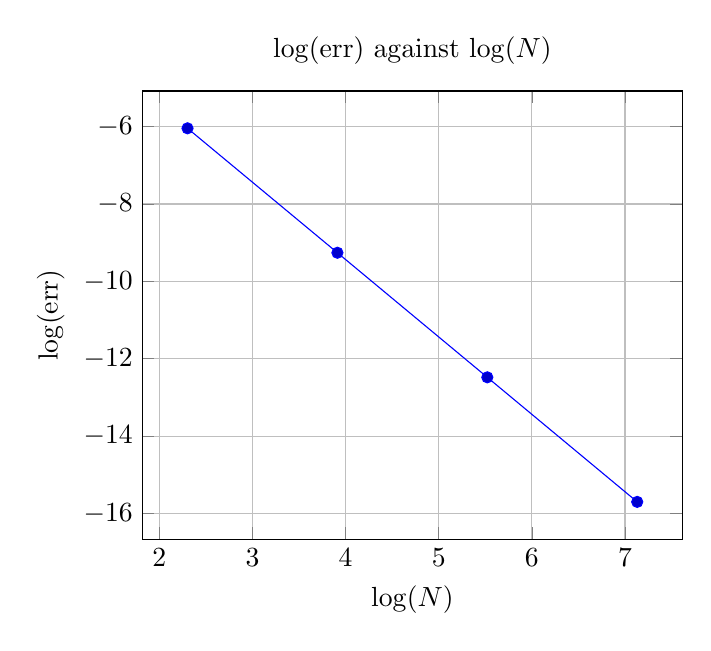
\begin{tikzpicture}
    \begin{axis}[
        xlabel={$\log(N)$},
        ylabel={$\log(\text{err})$},
        title={$\log(\text{err})$ against $\log(N)$},
        grid=major,
    ]
        \addplot coordinates {
            (2.302585092994, -6.045346786600)
            (3.912023005428, -9.260707644136)
            (5.521460917862, -12.479442011216)
            (7.130898830296, -15.698311799022)
        };
    \end{axis}
  \end{tikzpicture}
\end{center}

\newpage
\qs{Double Integral over a Bounded Region}{
  Evaluate 
  $$
    \iint_D x(y-1) \d A
  $$
  where $D$ is the region bounded by $y_1=1-x^2$ and $y_2=x^2-3$ in two ways using different orders of integration.
  %Hint: for one of them you may need to break up the integral into two parts.
}
\sol \\
The first way we'll do this is by finding the bounds of the double integral with respect to $x$ and $y$ and then integrating normally. \\

On the domain where the region is bound, $y_2 < y_1$. Hence the upper bound will be $y_1 = 1 - x^2$, and the lower bound will be $y_2 = x^2- 3$. \\
The domain itself will be bounded by the two points where $y_1$ meets $y_2$.
$$
  y_1 = y_2 \iff 1 - x^2 = x^2 - 3 \iff 0 = 2x^2 - 4 \iff 0 = x^2 - 2 \iff x^2 = 2 \iff x = \pm\sqrt{2}
$$
Therefore, the lower bound is $x_2 = -\sqrt{2}$ and the upper bound is $x_1 = \sqrt{2}$. \\
Now we can substitute the variables and find the integral.
\begin{align*}
  I &= \iint_D x(y-1) \d A \\
    &= \int_{-\sqrt{2}}^{\sqrt{2}}\int_{x^2 - 3}^{1 - x^2} x(y-1)\ \d y\d x \\
    &= \int_{-\sqrt{2}}^{\sqrt{2}} x \int_{x^2 - 3}^{1 - x^2} y-1\ \d y\d x \\
    &= \int_{-\sqrt{2}}^{\sqrt{2}} x \bracks{\sqbracks{\frac{1}{2}y^2}_{x^2 - 3}^{1 - x^2} - \sqbracks{\vphantom{\frac{1}{2}}y}_{x^2 - 3}^{1 - x^2}} \d x \\
    &= \int_{-\sqrt{2}}^{\sqrt{2}} x \bracks{\sqbracks{\frac{1}{2}\bracks{{1 - x^2}}^2 - \frac{1}{2}\bracks{x^2 - 3}^2} - \sqbracks{\vphantom{\frac{1}{2}}(1 - x^2) - (x^2 - 3)}} \d x \\
    &= \int_{-\sqrt{2}}^{\sqrt{2}} x \bracks{\bracks{\frac{1 - 2x^2 + x^4 - x^4 + 6x^2 - 9}{2}} - \bracks{1 - x^2 - x^2 + 3}} \d x \\
    &= \int_{-\sqrt{2}}^{\sqrt{2}} x \bracks{2x^2 - 4 + 2x^2 - 4} \d x \\
    &= \int_{-\sqrt{2}}^{\sqrt{2}} x \bracks{4x^2 - 8} \d x \\
    &= \int_{-\sqrt{2}}^{\sqrt{2}} 4x^3 - 8x\ \d x \\
    &= \sqbracks{x^4}_{-\sqrt{2}}^{\sqrt{2}} - \sqbracks{4x^2}_{-\sqrt{2}}^{\sqrt{2}} \\
    &= \bracks{\sqrt{2}^4 - \bracks{-\sqrt{2}}^4} - \bracks{4\bracks{\sqrt{2}}^2 - 4\bracks{-\sqrt{2}}^2} \\
    &= \bracks{4 - 4} - \bracks{8 - 8} \\
  \tf I &= 0
\end{align*}

\newpage
Next, we'll evaluate the integral by expressing $D$ as a Type II region. To do that, 
$$
D' = {(x,y) : c \leq y \leq d, h_1(y) \leq x \leq h_2(y)}
$$
Finding the min and max of $y$ in $D$ is finding $c$ and $d$ respectively. Because $y = 1 - x^2$ and $ y = x^2 - 3$ are quadratics, we know that either the min or max occurs on the axis of symmetry, $x = \frac{-b}{2a}$.
\begin{align*}
    y = 1 - x^2 &&&& y = x^2 - 3 \\
    && b=0 \implies x = 0 & \\
    y = 1 - 0^2 &&&& y = 0^2 - 3 \\
    y = 1 &&&& y = -3 \\
    && \therefore c = -3, \ d = 1
\end{align*}
Now we need to find $h_1 (y)$ and $h_2(y)$.
\begin{align*}
    x^2 - 3 &\leq y \\
    x^2 &\leq y - 3 \\
    \implies -\sqrt{y - 3} &\leq \ x^2 \leq \sqrt{y - 3} \\
    \\
    y &\leq 1 - x^2 \\
    y - 1 &\leq -x^2 \\
    1 - y &\geq x^2 \\
    \implies -\sqrt{1 - y} &\leq x \leq \sqrt{1 - y} 
\end{align*}
So, $x$ is bounded above by 2 functions and bounded below by 2 functions. If we find where they intersect, we can introduce a piecewise function that correctly defines an equivalent domain to $D$. 
\begin{align*}
    \text{Bounded above:}\\
    \sqrt{1 - y} &= \sqrt{y + 3} \\
    1 - y &= y + 3 \\
    2y &= -2 \\
    y &= -1 \\ \\
    \text{Bounded below:} \\
    -\sqrt{1 - y} &= -\sqrt{y + 3} \\
    1 - y &= y + 3 \\
    y &= -1
\end{align*}
So between $-3$ and $-1$, $x$ is bounded by $\pm \sqrt{y + 3}$ and between $-1$ and $1$, $x$ is bounded by $\pm \sqrt{1 - y}$. We can express each as its own region.

$$
B = {(x, y): -3 \leq y \leq -1, -\sqrt{y +3} \leq x \leq \sqrt{y + 3}}
$$

$$
C = {(x, y): -1 \leq y \leq 1, -\sqrt{1-y} \leq x \leq \sqrt{1 - y}}
$$
Now we can express $D'$ as a union between these 2 regions.
$$
D' = B \cup C
$$
\begin{align*}
    I = \iint_D x(y-1) \d A &= \iint_{D'}x(y-1)\d A \\
    I &= \iint_B x(y-1)dA + \iint_Cx(y-1)\d A \\
    &= \int_{-3}^{-1} \int_{-\sqrt{y + 3}}^{\sqrt{y+3}} x(y-1) \d x\d y + \int_{-1}^{1} \int_{-\sqrt{1-y}}^{\sqrt{1-y}} x(y-1) \d x\d y \\
    &= \int_{-3}^{-1} (y-1)\int_{-\sqrt{y + 3}}^{\sqrt{y+3}} x \d x \ \d y + \int_{-1}^{1} (y-1)\int_{-\sqrt{1-y}}^{\sqrt{1-y}} x \d x \ \d y \\
    &= \int_{-3}^{-1} (y-1) \Big[ \frac{1}{2} x^2 \Big]_{-\sqrt{y + 3}}^{\sqrt{y + 3}}\ dy + \int_{-1}^{1} (y-1) \Big[ \frac{1}{2} x^2 \Big]_{-\sqrt{1-y}}^{\sqrt{1 -y}}\ \d y \\
    &= \int_{-3}^{-1} (y-1) (\frac{1}{2}(\sqrt{y+3})^2 - \frac{1}{2}(-\sqrt{y+3})^2 \d y + \int_{-1}^{1} (y-1) (\frac{1}{2}(\sqrt{1-y})^2 - \frac{1}{2}(-\sqrt{1-y})^2 \d y \\
    &= \int_{-3}^{-1} (y-1) (\frac{y+3}{2}  - \frac{y + 3}{2}) dy + \int_{-1}^{1} (y-1) (\frac{1-y}{2}  - \frac{1-y}{2}) \d y \\
    &= \int_{-3}^{-1} (y-1) \cdot 0 dy + \int_{-1}^{1} (y-1) \cdot 0 \d y \\
    &= \int_{-3}^{-1} 0 \d y + \int_{-1}^{1} 0\d y \\
  \tf I &= 0 \\
\end{align*}
So, we successfully defined a Type II region, and used $\d x\d y$ instead of $\d y\d x$, and got the same answer for the integral, $0$.

\newpage
\section*{Appendix 1 - Table and Plot Code}
\begin{lstlisting}[language=TeX]
\begin{center}
  \begin{tabular}{l|rrr}
    \multicolumn{1}{c|}{$N$} & \multicolumn{1}{c}{Approx Volume} &
    \multicolumn{1}{c}{$\log(N)$} &
    \multicolumn{1}{c}{$\log(\text{err})$} \\ \hline
    10    & 1.716707432355  & 2.302585092994 & -6.045346786600  \\
    50    & 1.718981203550  & 3.912023005428 & -9.260707644136  \\
    250   & 1.719072487504  & 5.521460917862 & -12.479442011216 \\
    1250  & 1.719076139400  & 7.130898830296 & -15.698311799022 \\
  \end{tabular}
  \vspace{2em}
  
  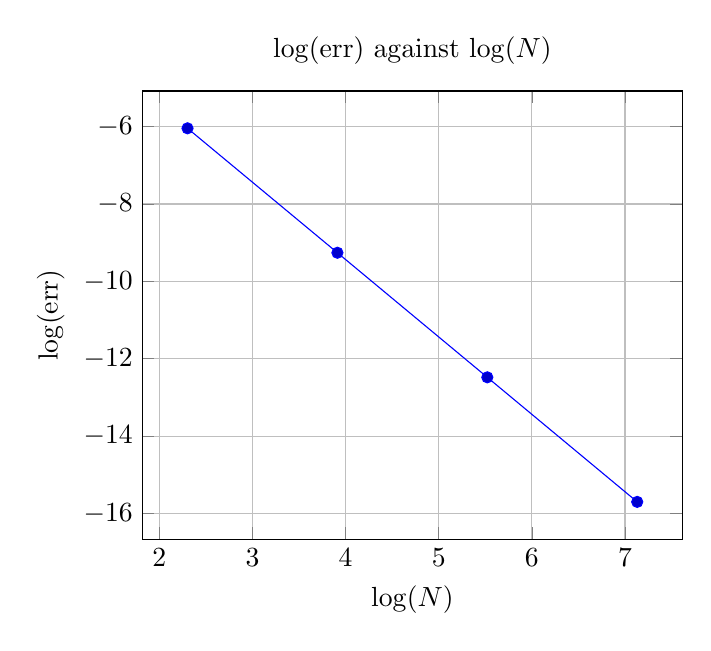
\begin{tikzpicture}
    \begin{axis}[
      xlabel={$\log(N)$},
      ylabel={$\log(\text{err})$},
      title={$\log(\text{err})$ against $\log(N)$},
      grid=major,
    ]
      \addplot coordinates {
        (2.302585092994, -6.045346786600)
        (3.912023005428, -9.260707644136)
        (5.521460917862, -12.479442011216)
        (7.130898830296, -15.698311799022)
      };
    \end{axis}
  \end{tikzpicture}
\end{center}
\end{lstlisting}


\end{document}
